\chapter{Scale, Control, and the Dubai Real-Estate Machine}

This lecture is not mathematical in the blackboard sense, but it is mathematical in a second and very real sense: it is about scale, control, operating depth, time horizon, and the conversion of narrative into asset value. The opening gives us a car, a skyline, and a startling number; the middle of the lecture translates that spectacle into a theory of real-estate wealth; and the ending compresses the whole structure into people, consistency, legacy, and faith. We will keep close to that order. The point is not to polish the interview into a generic business sermon. The point is to follow its own progression from visible wealth to the machinery that makes such wealth possible.

\section{Abnormal Scale as the Opening Fact}

The lecture opens with deliberate violence. Before we are given a theory, we are given a Bugatti, a claim to be one of the biggest real-estate developers in the world, and then a coarse numerical marker for the scale at stake:
\begin{equation}
Y_{\max} \approx \$5 \times 10^{9}.
\end{equation}
Here \(Y_{\max}\) denotes the self-reported largest amount of money made in a single year.

\begin{remark}
The transcript gives this number as an off-the-top-of-the-head range. We therefore keep it approximate and do not pretend to know whether it refers to profit, income, realized gains, or some broader business measure.
\end{remark}

That caution matters, but it does not weaken the opening move. The number is not introduced for accounting precision. It is introduced to set the scale of the conversation. Only after the number is on the page does the host widen the frame and say, in effect, that this is Dubai: a city where billion-dollar deals are made over coffee, where single visions shape skylines, and where wealth is operating on a different order of magnitude.

So the lecture begins with a very clear structure. First we are shocked. Then we are told that the shock is not accidental; it belongs to a place. Finally we are told that the place is not merely decorative. It is the field in which the later questions about entrepreneurship, real estate, and wealth are supposed to make sense.

\section{The Site as Proof}

The interview does not remain at the level of city myth. The host travels to the Bugatti Residences and keeps insisting on the location. We are not simply in Dubai; we are standing at one of Mohamed Benghadi's projects, described in the transcript as the first Bugatti Residence in the world, with the Burj Khalifa visible nearby as an anchor of urban scale.

This is a very important narrative move. Before the lecture asks for theory, it asks for proof. The building is not background. It is evidence. The host wants the viewer to see that the speaker is not offering a detached opinion about wealth. He is speaking from inside a product that already exists in the world.

\subsection{Question \& Answer}

\paragraph{Question.} How does someone become credible enough to build with one of the biggest luxury brands in the world?

\paragraph{Answer.} Mohamed's first answer is not technical. It is temperamental. He says that passion goes into it, that one has to be obsessed, that one wakes up every day obsessed with goals and willing to grind. This comes before finance, before structure, and before design. The lecture wants us to see that a branded skyscraper is not born first from clever positioning. It begins from obsession sustained long enough to become visible to the world.

The answer remains partly biographical. He recalls Bugatti posters in his room as a child and says he never would have imagined achieving something like this. But the lecture does not stay at the level of childhood dream. It immediately uses that answer to pivot toward a broader operating question: why this city, and why this environment?

\section{Entrepreneurial Atmosphere, Failure, and the Choice of Real Estate}

Mohamed says he never left the UAE because, in his view, it is the best place in the world. When pressed, he explains this in institutional language: the city has entrepreneurial flair, and the leadership has helped create an atmosphere in which an entrepreneur can build a billion-dollar business. That answer does real work in the lecture. It shifts us from private will to public setting.

But the lecture does not allow the setting to become a fairy tale. The next insertion is failure. The host asks whether there were many no's, many downsides, many failures. Mohamed answers immediately: plenty. The more successful one becomes, he says, the more one realizes that failure and rejection are normal. Success therefore cannot mean the absence of friction. It must mean the capacity to navigate through rejection toward the answer one wants.

Only after that preparatory work does the lecture ask its first major economic question: why real estate?

\subsection{Question \& Answer}

\paragraph{Question.} Why do wealthy people keep ending up in real estate?

\paragraph{Answer.} Mohamed's claim is strong: everyone who makes a lot of money ends up buying real estate. In the lecture's shorthand, we can write
\begin{equation}
W_{\text{large}} \Longrightarrow A_{\text{RE}},
\end{equation}
where \(W_{\text{large}}\) denotes large accumulated wealth and \(A_{\text{RE}}\) denotes a significant real-estate allocation.

We should not read this as a universal theorem. It is a practical rule of the interview. The mechanism he gives is equally clear:
\begin{equation}
\text{tangibility} + \text{lower volatility} + \text{risk-manageability}
\Longrightarrow
\text{real-estate preference}.
\end{equation}
Real estate is, in his language, solid. One can touch it, feel it, see it, smell it. It is treated as less volatile than many alternatives, and therefore as a safer place to store or compound wealth.

\paragraph{Claim.} Real estate is not merely a way to make money. It is also the place where money likes to come to rest.

\paragraph{Mechanism.} The asset has physicality, perceived stability, and a risk profile that wealthy people find legible.

This is the first real spine of the lecture. We have moved from spectacle to asset theory.

\section{Diversification by Going Deeper, Not Wider}

The next move is more subtle and, in many ways, more powerful. When asked about diversification, Mohamed says that he did diversify, but learned a hard lesson: diversification does not always mean going into another sector. One can diversify inside a single sector. The name he gives for this is vertical integration.

\begin{definition}
In the language of this lecture, vertical integration means that the developer does not merely conceive and sell projects. He progressively takes ownership of the chain that builds them: construction, workforce, factories, and the relevant production infrastructure.
\end{definition}

So the interview's redefinition of diversification may be written as
\begin{equation}
\text{diversification} \neq \text{necessarily new sector},
\qquad
\text{diversification} = \text{deeper control along one chain}.
\end{equation}

Mohamed then gives concrete content to that claim. The company became completely vertically integrated as a developer. It built a full construction company. It has seven factories, with joinery, aluminum, and steel named explicitly in the transcript. The middle argument of the lecture can therefore be written in a compact operational form:
\begin{equation}
V_{\text{int}}
=
\{\text{construction},\ \text{in-house workforce},\ \text{factories}\}
\Longrightarrow
(\text{speed},\ \text{quality},\ \text{cost control}).
\end{equation}

\begin{figure}[h]
\centering
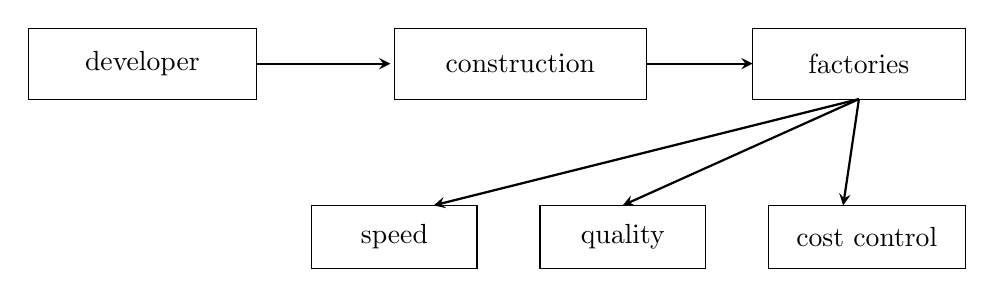
\begin{tikzpicture}[x=1cm,y=1cm,>=stealth]
\node[draw, rectangle, minimum width=2.9cm, minimum height=0.9cm] (dev) at (0,0) {developer};
\node[draw, rectangle, minimum width=3.2cm, minimum height=0.9cm] (con) at (4.8,0) {construction};
\node[draw, rectangle, minimum width=2.7cm, minimum height=0.9cm] (fac) at (9.1,0) {factories};

\draw[->, thick] (1.45,0) -- (3.15,0);
\draw[->, thick] (6.4,0) -- (7.75,0);

\node[draw, rectangle, minimum width=2.1cm, minimum height=0.8cm] (spd) at (3.2,-2.2) {speed};
\node[draw, rectangle, minimum width=2.1cm, minimum height=0.8cm] (qua) at (6.1,-2.2) {quality};
\node[draw, rectangle, minimum width=2.5cm, minimum height=0.8cm] (cost) at (9.2,-2.2) {cost control};

\draw[->, thick] (9.1,-0.45) -- (3.7,-1.8);
\draw[->, thick] (9.1,-0.45) -- (6.1,-1.8);
\draw[->, thick] (9.1,-0.45) -- (8.9,-1.8);
\end{tikzpicture}
\end{figure}

We should read this figure as an editorial transcription of the lecture's middle claim. The developer who owns more of the production chain is not merely larger. He is more agile.

\subsection{Question \& Answer}

\paragraph{Question.} What does diversification mean if leaving the sector is not the right move?

\paragraph{Answer.} It means taking the sources of uncertainty inside the house. One does not flee the chain; one thickens one's control over it. The lecture is explicit about the payoff: speed, quality, and cost.

This is a very different picture of growth from the usual entrepreneurial temptation to scatter attention across unrelated businesses. Mohamed's language is memorable here. Rather than getting distracted in different sectors, they chose to serve one single monstrosity of a business.

\section{Building Without the Full Picture}

At this point the host asks the natural question. If the final machine contains development, construction, workforce, and factories, how does one actually get there? Surely nobody begins on day one with the whole picture.

Mohamed's answer is one of the best parts of the lecture. He says that in business one never has the full picture from day one. One must start and navigate through. He then uses the image of a bee beginning its day without a full plan, and the related image of survival in a stormy sea: one either drowns or swims.

This is not a polished planning doctrine. It is an iterative doctrine.

\subsection{Question \& Answer}

\paragraph{Question.} How do we scale when we do not yet know the full map from day one?

\paragraph{Answer.} We start, encounter bottlenecks, learn, and internalize what the business later reveals that it needs. A cautious mathematical rendering of that progression is
\begin{align}
V_0 &= \{\text{development}\},\\
V_1 &= V_0 \cup \{\text{construction}\},\\
V_2 &= V_1 \cup \{\text{factories}\},\\
V_{n+1} &= V_n \cup \{\text{next bottleneck to internalize}\}.
\end{align}

This is not stated on screen in this form, and we should say so. But it is the cleanest compact notation for what the interview actually describes. The company does not begin as a finished empire. It expands by absorbing the next necessary function.

A second way to write the same logic is as a navigation loop:
\begin{equation}
\text{start} \to \text{navigate} \to \text{fail} \to \text{fix} \to \text{figure out a way}.
\end{equation}

\paragraph{Worked example.} Suppose the initial business contains only development. Then outside contractors determine build speed and production quality. Once construction is internalized, one source of delay and quality uncertainty is reduced. Once factories are added, additional supply bottlenecks are pulled inward. Each step changes the geometry of control. The important point is that the sequence is discovered operationally. It is not fully known in advance.

This is why the bee and the storm metaphors matter. They are not ornamental. They tell us how the speaker wants uncertainty to be understood: not as evidence that action should wait, but as the condition under which action becomes intelligent.

\section{What the Product Proves}

The lecture now returns to the building, and the return is quantitative. The building is no longer just a branded location. It becomes a ledger of scale:
\begin{align}
L_{\text{cladding}} &= 13\,\mathrm{km},\\
N_{\text{stories}} &= 46, \qquad N_{\text{units}} = 180,\\
A_{\text{penthouse}} &\approx 50{,}000\,\mathrm{ft}^2, \qquad N_{\text{car elevators}} = 2,\\
P_{\text{penthouse}} &= 750 \times 10^{6}\,\mathrm{AED}
\approx 2 \times 10^{8}\,\mathrm{USD}.
\end{align}

These numbers matter because they convert business doctrine into visible product. The transcript also adds texture: the penthouse is a triplex; it contains a cinema and cigar lounge; there is a French Riviera inspired beach high in the building; and the units are described as bespoke, each with a distinct layout and interior scheme.

\paragraph{Anecdote.} The host walks the site and reacts to the extravagance.

\paragraph{Claim.} The best product speaks for itself.

\paragraph{Mechanism.} When design, construction speed, and brand narrative are all aligned, the building becomes its own marketing engine:
\begin{equation}
Q_{\text{product}} \uparrow
\Longrightarrow
M_{\text{required}} \downarrow,
\end{equation}
where \(Q_{\text{product}}\) denotes product quality and \(M_{\text{required}}\) the amount of verbal persuasion still needed to move the offer.

The lecture is careful here. Mohamed does not deny marketing; he says they market globally. But he insists that the best companies are the ones whose products market themselves. The site walk is the proof of that sentence.

The same logic extends to design. When the host asks what goes into great design, Mohamed answers with storytelling, brand narrative, the name of the project, the architecture, the interiors, the exterior, the amenities, and above all the lifestyle being built for a specific audience. In other words, design is not decoration added to a commodity. It is a narrative structure through which the right buyer comes to see value.

\section{People, Time, and the Compounding Loop}

Once the lecture has established scale, asset choice, and product, it turns toward people. Mohamed quotes a managerial hierarchy of sixes, sevens, eights, nines, and tens, insisting that truly great organizations are built out of nines and tens:
\begin{equation}
R_{\text{talent}} \in \{6,7,8,9,10\}.
\end{equation}
But the important line is not the scale itself. It is the test that follows: if he has to tell someone what to do, that person is not in the right place.

This becomes a stronger doctrine when he explains the Arabic saying that once the chick is born it knows how to walk, and once the duckling is born it knows how to swim. The worker who belongs in the role should not merely wait for instructions. That person should know what to do and, ideally, should know more than the boss about the specialized craft in question.

So the lecture rejects micromanagement, but not involvement. Mohamed calls the alternative passion management: be involved in everything if necessary, but empower specialized people to do their work at a higher level than one's own.

\subsection{Question \& Answer}

\paragraph{Question.} What separates a merely capable operator from a builder who compounds for decades?

\paragraph{Answer.} The lecture gives a three-part answer.

First, the builder assembles self-starting people rather than instruction-dependent people.

Second, the builder plays a long game. The host introduces Reid Hoffman's phrase about never playing a one-year game and only playing a ten-year game:
\begin{equation}
T_{\text{game}} = 10\ \text{yr}.
\end{equation}
Mohamed then pushes further. For him there is no fixed term at all. Work becomes lifestyle, daily routine, and permanent discipline.

Third, the builder turns failure into recurrence rather than catastrophe. This is why consistency becomes the central variable:
\begin{equation}
S \propto C \cdot T,
\end{equation}
where \(S\) denotes success, \(C\) consistency, and \(T\) sustained time. Again, we do not read this as a statistical law. We read it as the lecture's condensed operating philosophy: less brilliant but more consistent people often outrun brilliant but inconsistent ones.

The closing formula of the lecture is even simpler:
\begin{equation}
\text{try} \to \text{fail} \to \text{learn} \to \text{fix} \to \text{try again}.
\end{equation}
This is the speaker's explicit five-step recipe, and it answers the host's later question about whether he could rebuild from zero. Yes, he says, because the process remains even if the possessions vanish.

The last compression of the lecture moves beyond technique. The speaker says one should leave behind something valuable: a project, a product, something that changes people's lives positively while also making money. That is the legacy claim. Then, when asked about faith, he gives another structure: one works to the limit, fails repeatedly, keeps following up, and sometimes the breakthrough arrives after prayer, as though a final external opening had been granted rather than engineered.

The interview does not try to prove that last point. It ends by locating the whole commercial machine inside a larger moral and theological horizon. For this lecture, that is the proper ending. Scale without faith would be too thin; faith without work would be sentimental. The interview wants both.

\section{Summary}

The argument of the lecture can now be read in a single line:
\begin{equation}
\text{scale} \to \text{asset choice} \to \text{control} \to \text{product} \to \text{people} \to \text{consistency} \to \text{legacy}.
\end{equation}
We begin with a Bugatti and a staggering annual figure, but we do not end there. We end with a more precise structure. Real estate is treated as the terminal asset of large wealth; diversification is redefined as deeper control along one chain; vertical integration produces speed, quality, and cost control; product quality lowers the burden of persuasion; self-starting people compound better than managed mediocrity; and success, in the long run, is tied to consistency, repeated correction, and the ability to continue after failure. That is the real mathematical payload of the interview.